\documentclass[12pt]{article}

\usepackage[T1]{fontenc}
\usepackage[utf8]{inputenc}
\usepackage[margin=1in]{geometry}
\usepackage{graphicx}
\usepackage{float}
\usepackage{amsmath}
\usepackage[table]{xcolor}
\usepackage{array}
\usepackage{pdflscape}

\definecolor{measured}{HTML}{009E73}
\definecolor{modelled}{HTML}{0072B2}
\definecolor{calculated}{HTML}{CC79A7}
\definecolor{approximation}{HTML}{E69F00}
\definecolor{proxy}{HTML}{56B4E9}
\definecolor{unresolved}{HTML}{D9D9D9}

\newcolumntype{L}[1]{>{\raggedright\arraybackslash}m{#1}}
\newcolumntype{C}[1]{>{\centering\arraybackslash}m{#1}}

\title{Many-body dynamics of the Radical Pair Mechanism}
\author{Sam Smart \and Lincoln D. Carr}
\date{}

\begin{document}

\maketitle

\section{Introduction}
Over the past 100 years, the field of quantum biology has grown through 2 eras of study in science. At first, a highly contended theoretical inception met with much criticism due to the unquantum nature of biological systems. 
The second era marked by experimental verification. We now have many commonly accepted quantum explanations for biological phenomena. Amongst others, the most famous being the effect of a radical pair of electrons within the body. 
And, as with the emergence of many quantum technologies in modern science, we see a shift to a third era for quantum biology, an era of engineerability and control. 

Understanding the radical pair mechanism as rich quantum many-body system beyond narrow biological parameter regimes and approximations becomes important in this 3rd era of quantum biology. We recognize that: *insert Dr Carr's section on cntral rotar models etc.*

We explore the system's dynamics in a high magnetic field strength regime far greater than the commonly-studied earth field strengths yet still biologically safe and lab achievable. 
Further study then goes into a many-body treatment of this sytem, studying nuclear many-body dynamics, dipolar, exchange, quadrupolar interaction effects and tracking entanglement through the system.

\clearpage
\begin{landscape}
\begin{table}[p]
    \centering
    \caption{Radical pair Hamiltonian parameter comparison.}
    \label{tab:radical-pair-hamiltonian-comparison}
    \scriptsize
    \setlength{\tabcolsep}{4pt}
    \renewcommand{\arraystretch}{1.18}
    \arrayrulecolor{black!25}
    \begin{tabular}{|L{1.00in}|L{1.25in}|C{0.70in}|C{0.75in}|C{0.90in}|L{1.70in}|L{1.85in}|}
        \hline
        \textbf{System} & \textbf{Radical pair} & \textbf{$r$ (\AA)} & \textbf{$J/h$ (MHz)} & \textbf{$\lvert D\rvert/h$ (MHz)} & \textbf{Dominant hyperfine $A/h$ (MHz)} & \textbf{Notes / provenance} \\
        \hline
        \textbf{Cryptochrome} & FAD$^{\bullet-}$ / TrpH$^{\bullet+}$ (TrpD) &
        \cellcolor{measured}21.2 $\pm$ 0.2 &
        \cellcolor{measured}$\sim$0.03 &
        \cellcolor{measured}5.46 $\pm$ 0.15 &
        \cellcolor{measured}FAD: ($-2.24$, $-2.02$, 47.48)\newline TrpD: (41.98, 43.69, 49.23) &
        Al Said 2022; RadicalPy/Evans 2024 \\
        \hline
        \textbf{Photolyase} & FADH$^{\bullet+}$ / CPD$^{\bullet-}$ &
        \cellcolor{modelled}\color{white}$\sim$3--8 &
        \cellcolor{approximation}$\sim 10^{1}$--$10^{3}$ &
        \cellcolor{approximation}$\sim$100--700 &
        \cellcolor{proxy}FADH$^{\bullet}$: ($-3$, $-24.60$, $-37.02$)\newline CPD$^{\bullet-}$: (16.01, 35.66, 57.88) &
        Schleicher 2010; Bernhard 1989; Maestre-Reyn 2018; Wilson 2011; Zhang 2017 \\
        \hline
        \textbf{Photosystem I / photosynthetic RC} & P700$^{\bullet+}$ / A1$^{\bullet-}$ &
        \cellcolor{calculated}25.4 $\pm$ 0.02 &
        \cellcolor{approximation}$\sim$0 &
        \cellcolor{measured}3.18 $\pm$ 0.01 &
        \cellcolor{measured}P700$^{\bullet+}$: (2.34, 2.34, 5.85), $\pm$0.2\newline A1$^{-}$: (1.37, 1.37, 1.96), $\pm$0.2 &
        K\"a\ss\ 1995; Hanely 1997; Link 2001 \\
        \hline
        \textbf{Bacterial reaction center} & P865$^{\bullet+}$ / QA$^{\bullet-}$ &
        \cellcolor{measured}28.4 $\pm$ 0.1 &
        \cellcolor{approximation}$\sim$0 &
        \cellcolor{calculated}2.27 $\pm$ 0.04 &
        \cellcolor{measured}P865$^{\bullet+}$: (2.37, 2.37, 6.42)\newline QA$^{\bullet-}$: (36, $-7$, $-7$) &
        Al Said 2022; K\"ass 1995; O'Malley 1998 \\
        \hline
        \textbf{Carotenoid-porphyrin-fullerene triad} & Carotenoid$^{\bullet+}$ / C60$^{\bullet-}$ &
        \cellcolor{modelled}\color{white}$\sim$30--36 &
        \cellcolor{modelled}\color{white}$\sim$0 &
        \cellcolor{calculated}$\sim$1--1.9 &
        \cellcolor{measured}Carotenoid$^{\bullet+}$: (16.23, 16.23, 16.23)\newline C60$^{\bullet-}$: (0, 0, 0) &
        Kerpal 2019; Lindoy 2020 \\
        \hline
        \textbf{AsLOV2 WT} & FMN$^{\bullet-}$ / C450$^{\bullet+}$ &
        \cellcolor{measured}$\sim$4.4 &
        \cellcolor{modelled}\color{white}$\sim$100 &
        \cellcolor{calculated}$\sim$600 &
        \cellcolor{modelled}\color{white}FMN$^{\bullet-}$: ($-11.68$, 292.63, $-10.47$)\newline C450$^{\bullet+}$: (48.52, 46.42, 53.03) &
        Salvia 2026; Maity 2025; Manian 2026 \\
        \hline
        \textbf{MagLOV} & FMN$^{\bullet-}$ / TrpH$^{\bullet+}$ &
        \cellcolor{modelled}\color{white}$\sim$15 &
        \cellcolor{calculated}$\sim$1.7 &
        \cellcolor{modelled}\color{white}$\sim$15.4 &
        \cellcolor{proxy}FMN$^{\bullet-}$: ($-10$, $-10$, 49)\newline TrpH$^{\bullet+}$: (41, 43, 49) &
        Antill 2026; Ross 2026; Abrahams 2026 \\
        \hline
    \end{tabular}

    \vspace{0.8em}
    \begin{minipage}{0.98\linewidth}
        \raggedright
        \textbf{Colour key:}\par\smallskip
        \setlength{\tabcolsep}{5pt}
        \renewcommand{\arraystretch}{1.35}
        \begin{tabular}{L{1.33in}L{1.33in}L{1.33in}L{1.33in}L{1.33in}L{1.33in}}
            \cellcolor{measured}Directly measured / directly reported &
            \cellcolor{modelled}\color{white}Literature model or fitted value &
            \cellcolor{calculated}Calculated here from reported literature value &
            \cellcolor{approximation}Magnitude approximation &
            \cellcolor{proxy}Proxy or analogue value &
            \cellcolor{unresolved}Unresolved / not available
        \end{tabular}
        \par\smallskip
        \emph{Cells with multiple pieces of provenance are coloured by the dominant or most conservative provenance category; details remain in the Notes / provenance column.}
    \end{minipage}
\end{table}
\end{landscape}
\clearpage

\section{Results}

\subsection{Dipole-Exchange Dynamics}
The first experiment we did was to add the exchange and dipolar interactions to the established 14 nuclei system. 
We started by simply adding the dipolar term. This interaction is well understood so our confidence in its implementation is high. 
The exchange interaction is less understood so this was treated as the independent variable against magnetosensitivity. We tested ranges inspired by the Efimova and Hore cancellation regions as well as a wide range of other values. 
The only values that showed magnetoreception were centered at the D=-3J region. We used these strengths going forward. 
\begin{figure}[H]
    \centering
    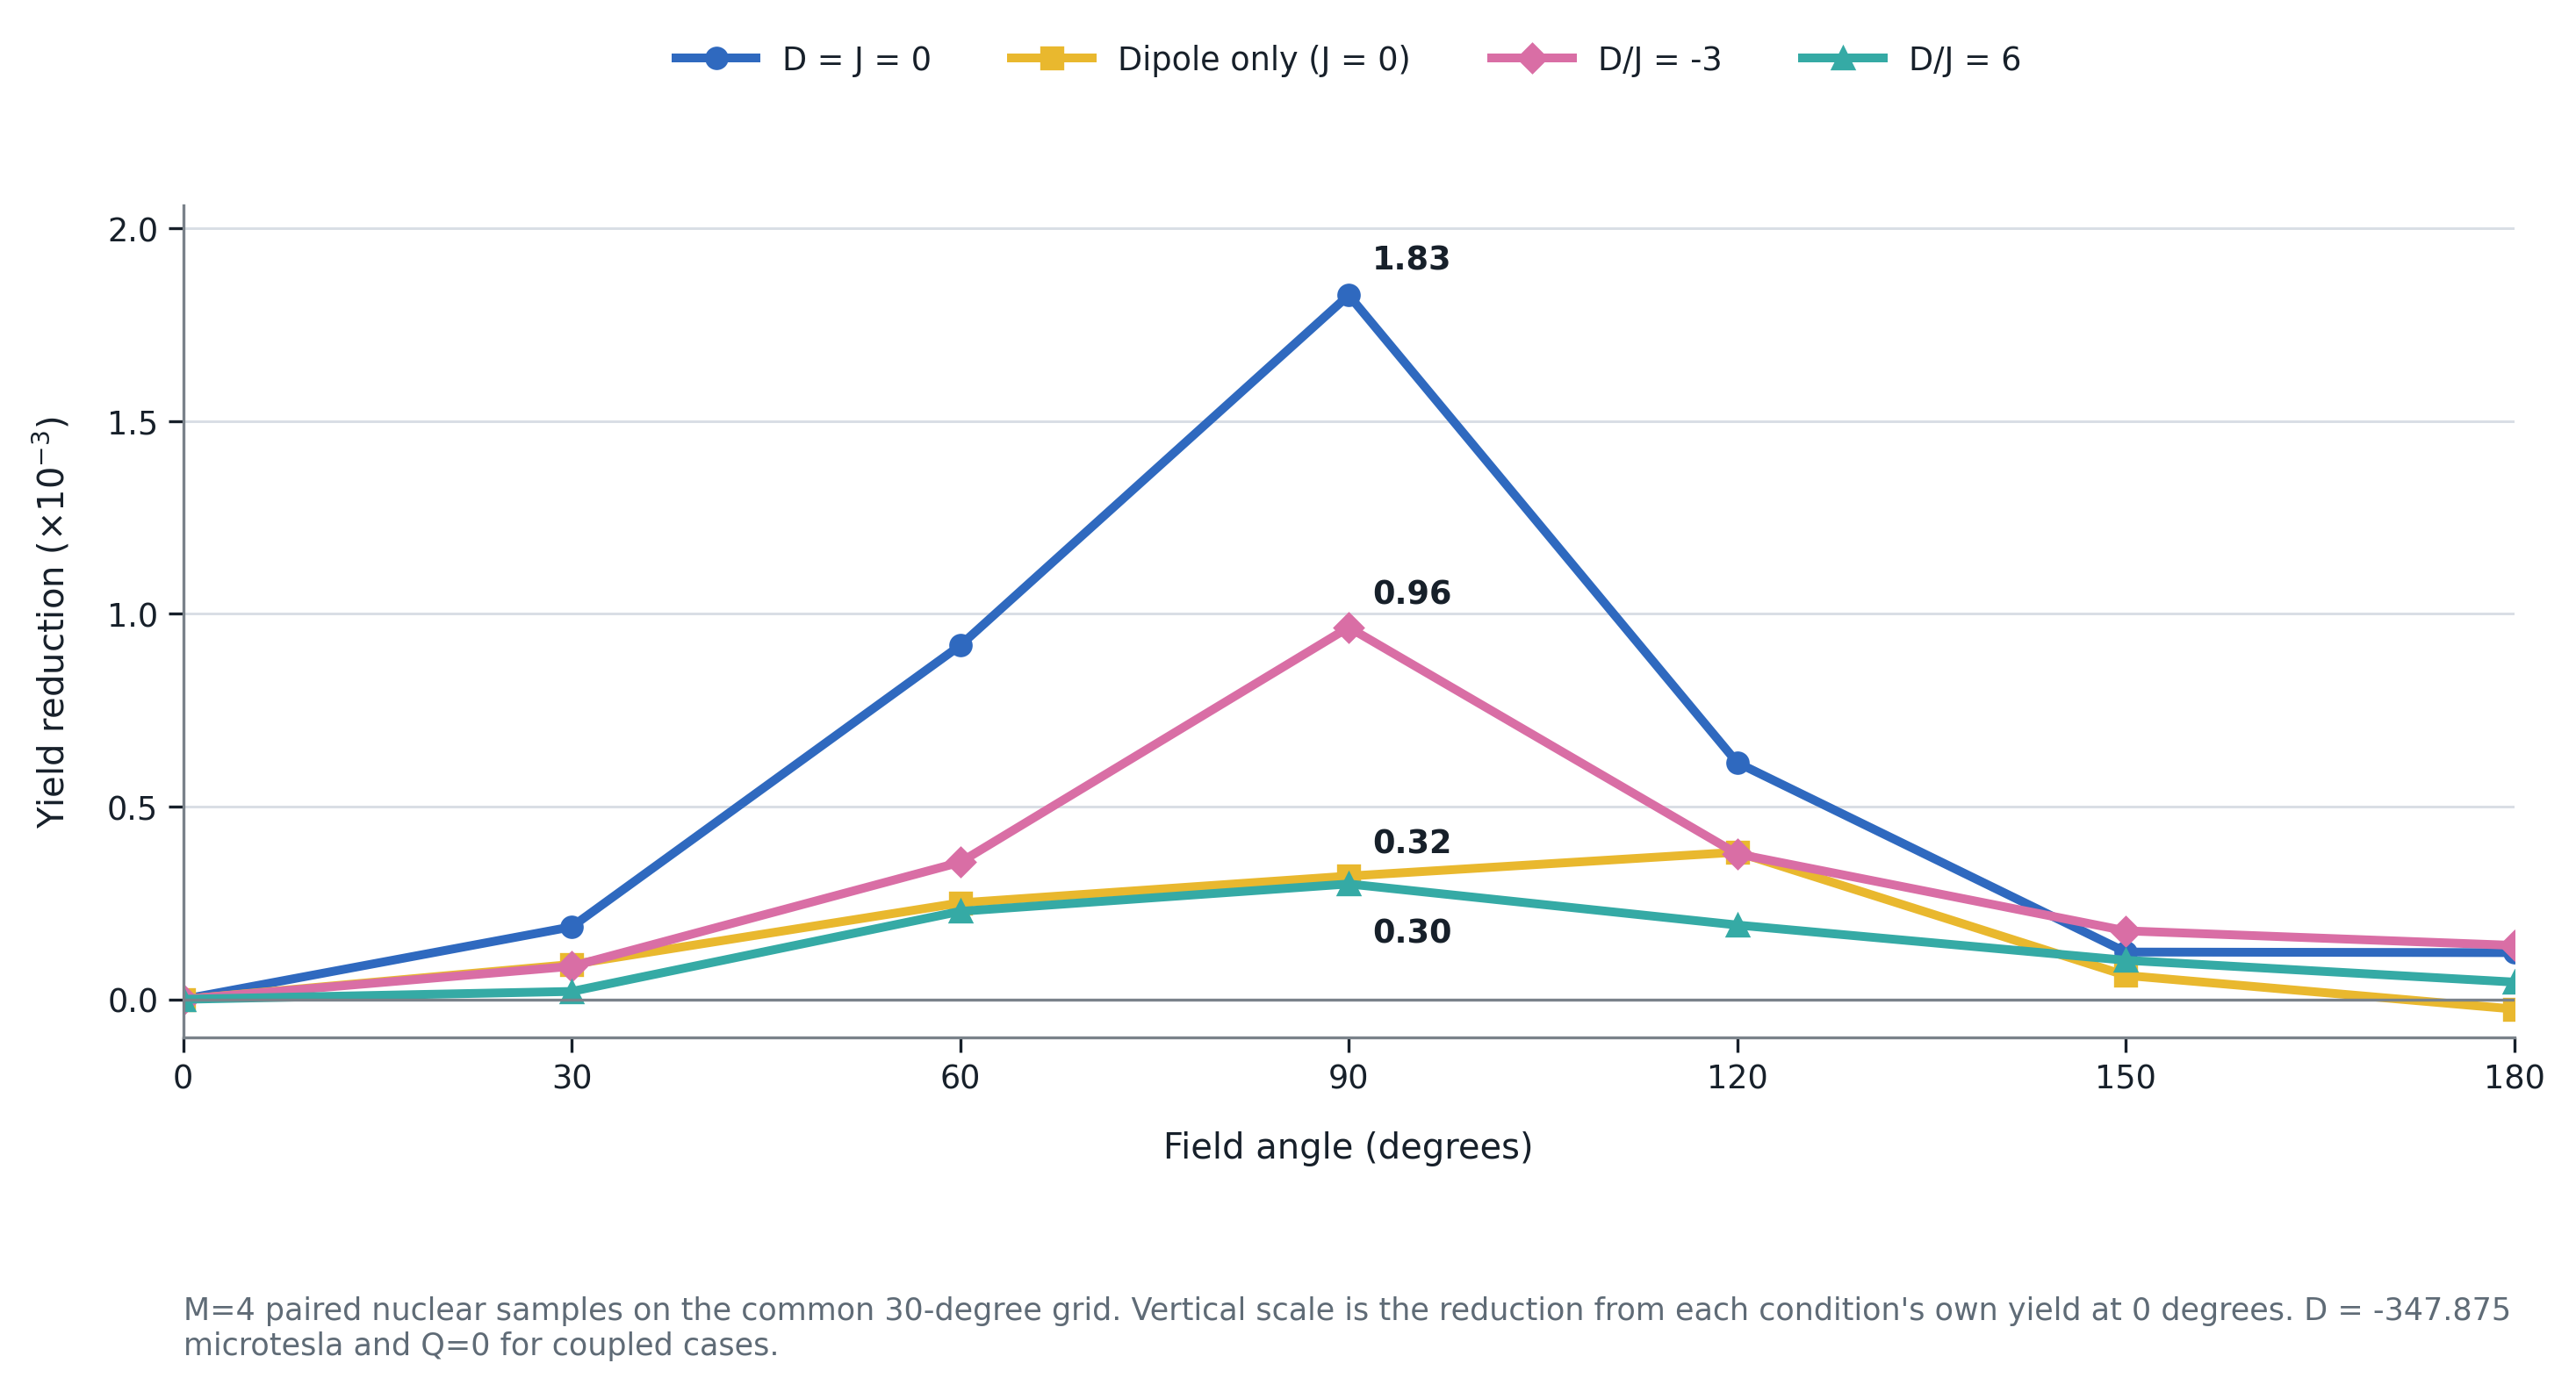
\includegraphics[width=\linewidth]{../figures/01-cancellation.png}
    \caption{Efimova--Hore dipolar cancellation curves.}
    \label{fig:efimova-hore-cancellation-curves}
\end{figure}
\subsection{High Field Dynamics}
\begin{equation}
    \begin{gathered}
        \begin{aligned}
            \hat{H} ={}&
            \underbrace{\gamma_e\,\mathbf{B}\cdot\hat{\mathbf{S}}}_{\text{magnetic field}}
            + \underbrace{\sum_{i=1}^{2}\sum_k \hat{\mathbf{S}}_i\cdot\mathbf{A}_{ik}\cdot\hat{\mathbf{I}}_{ik}}_{\text{hyperfine}} \\
            &+ \underbrace{D\left[(\hat{\mathbf{S}}\cdot\mathbf{n})^{2} - \frac{\hat{\mathbf{S}}^{2}}{3}\right]}_{\text{dipolar}}
            \underbrace{{}- J\left(\hat{\mathbf{S}}^{2} - \mathbf{1}\right)}_{\text{exchange}}
            + \underbrace{\sum_{i=1}^{2}\sum_k \hat{\mathbf{I}}_{ik}\cdot\mathbf{Q}_{ik}\cdot\hat{\mathbf{I}}_{ik}}_{\text{quadrupolar}},
        \end{aligned} \\
        \hat{\mathbf{S}} = \hat{\mathbf{S}}_1 + \hat{\mathbf{S}}_2,
        \qquad \lvert\mathbf{n}\rvert = 1,
        \qquad \hbar = 1.
    \end{gathered}
    \label{eq:radical-pair-hamiltonian}
\end{equation}

\begin{samepage}
We use the cancellation condition $D=-3J$. At an electron separation of $r=2\,\mathrm{nm}$, the field-equivalent coupling strengths are $D=-347MHz\,\mu\mathrm{T}$ and $J=116MHz\,\mu\mathrm{T}$. We set $Q=2-4MHz$ and neglect the nuclear Zeeman interaction.

\end{samepage}

The initial state consists of singlet electrons and an approximately maximally mixed nuclear bath. We use an evolution time of $T=5\,\mu\mathrm{s}$ and retain the seven strongest nuclei on each radical. The hyperfine coupling tensors are taken from density functional theory (DFT) calculations [ref]. Error bars are included but are small.

We scale the external magnetic field from Earth's field strength of $50\,\mu\mathrm{T}$ to $100\,\mathrm{mT}$, cited as a biologically safe extreme, and also consider $400\,\mathrm{mT}$ as an extreme maximum [refs].

\begin{figure}[H]
    \centering
    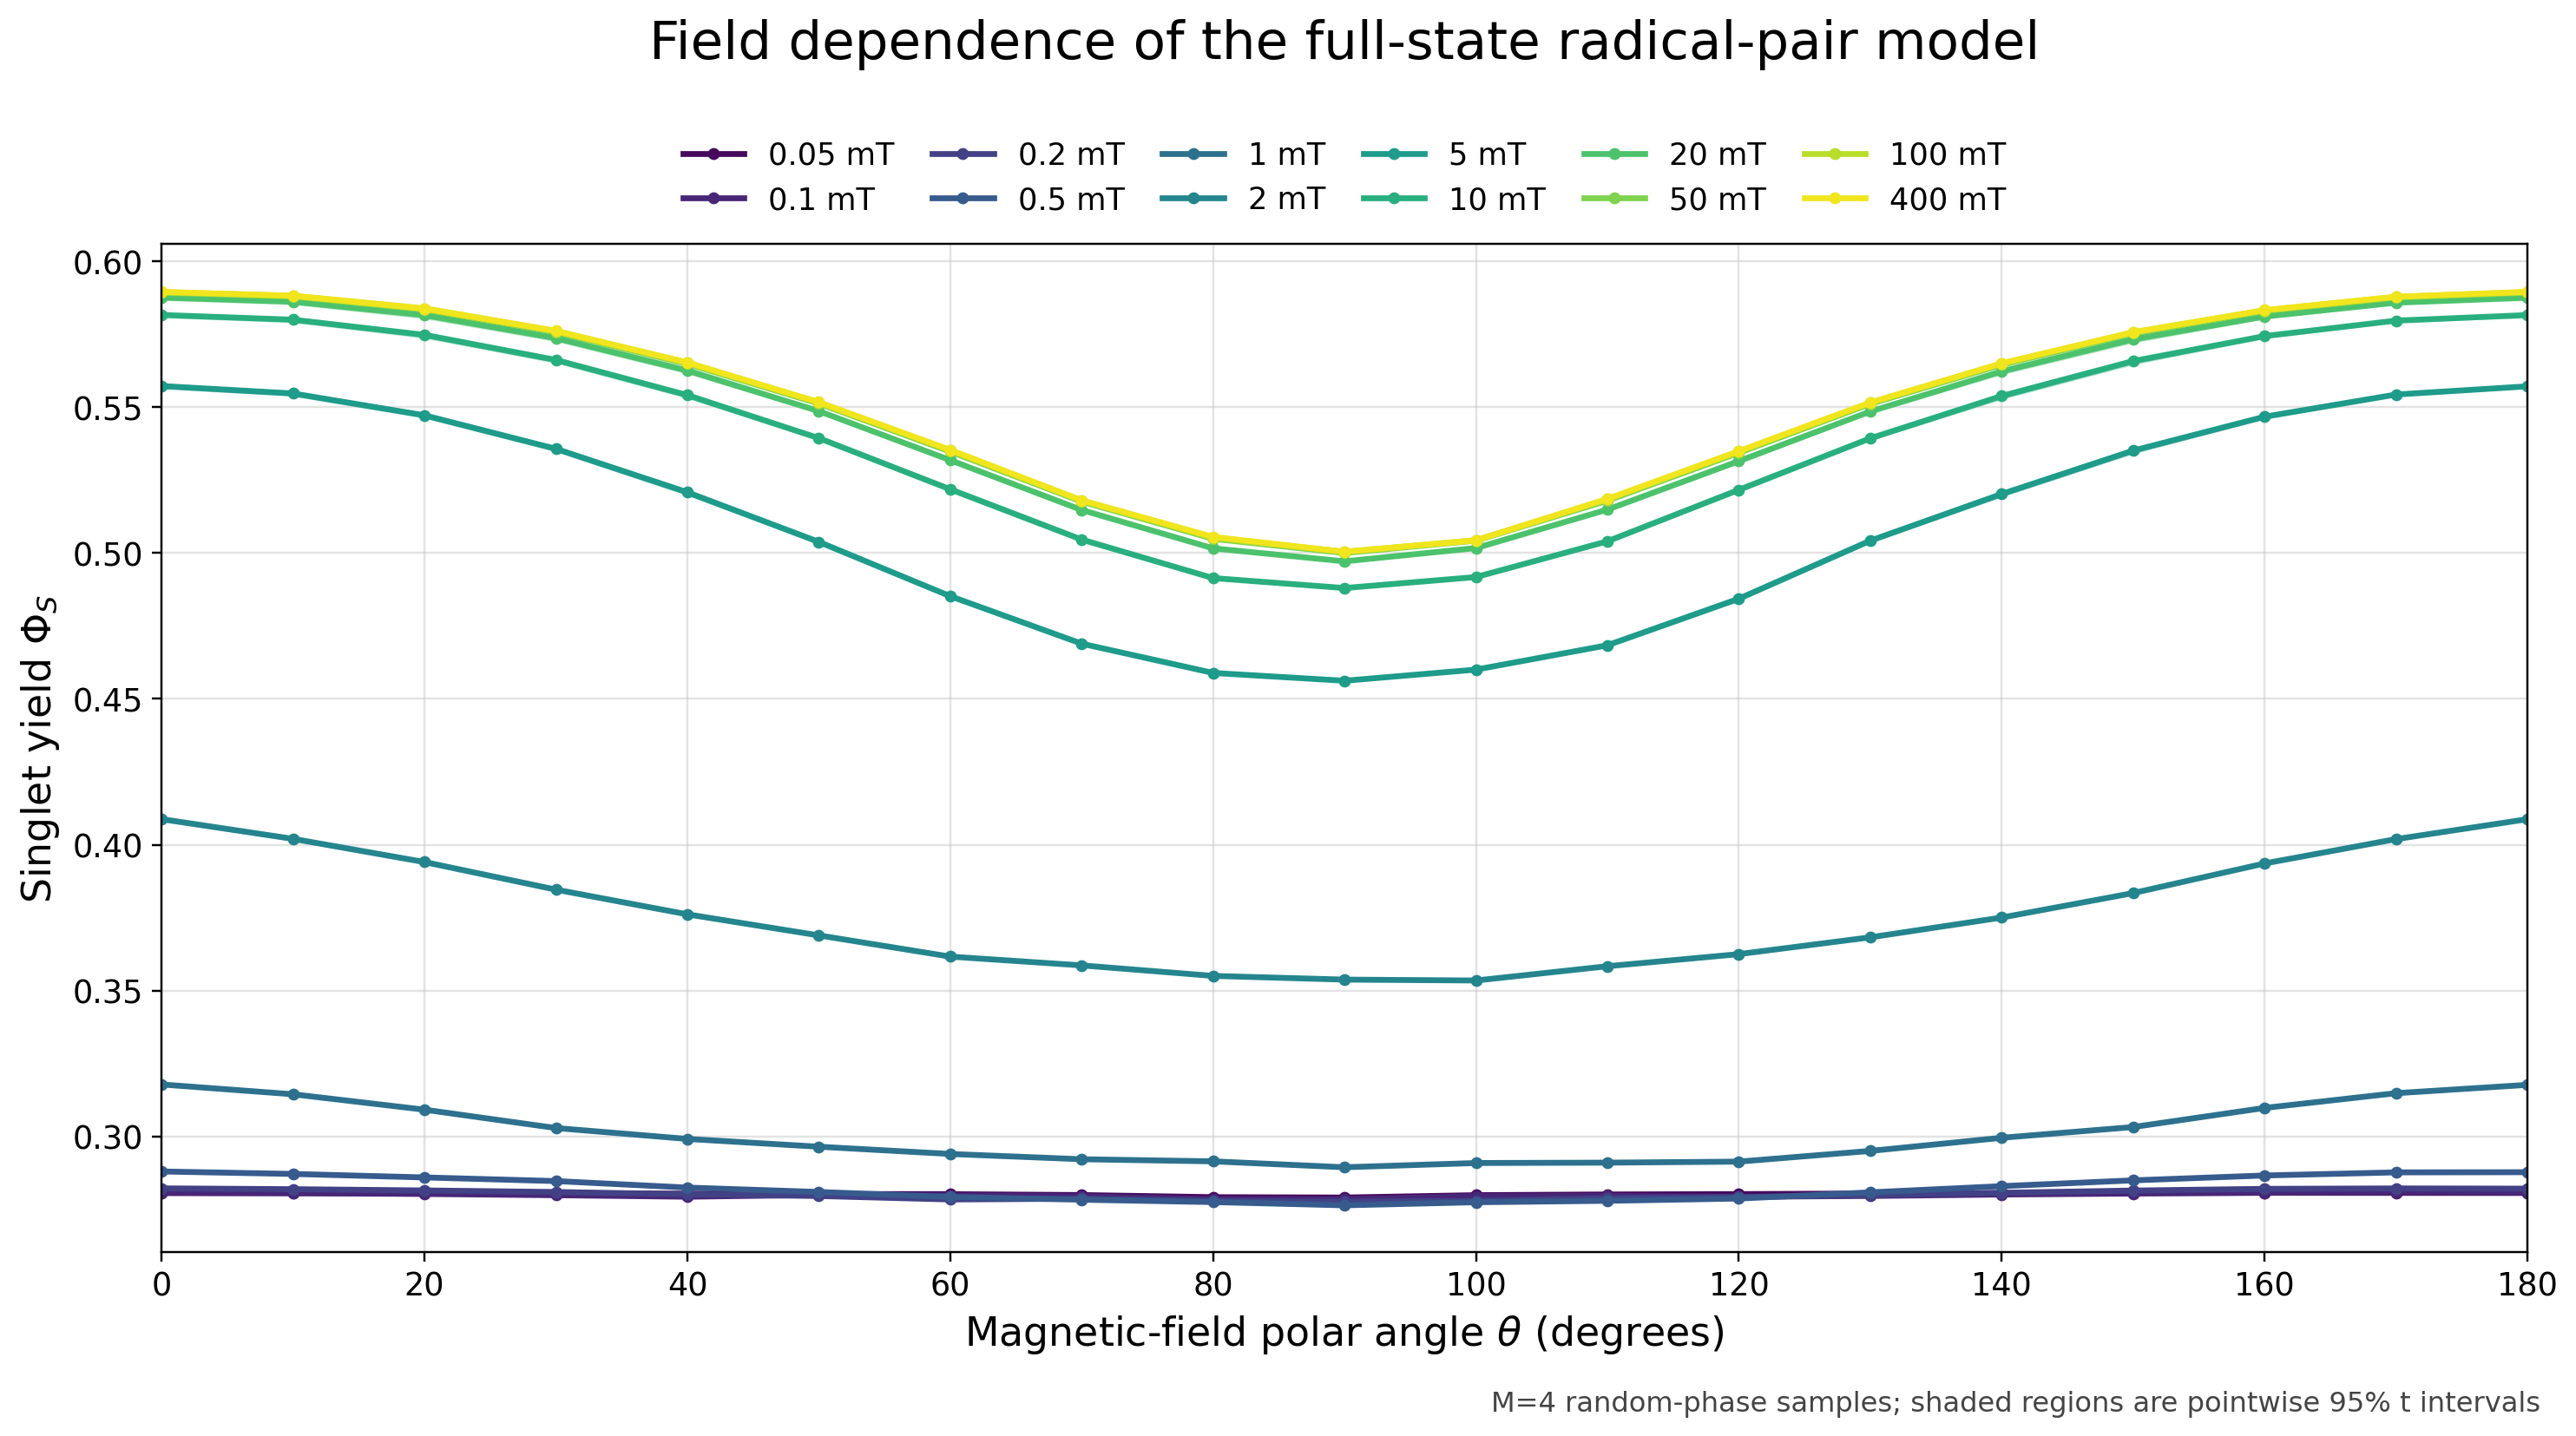
\includegraphics[width=\linewidth]{../figures/02-field-sweep.png}
    \caption{Field scaling.}
    \label{fig:field-scaling}
\end{figure}
\begin{figure}[H]
    \centering
    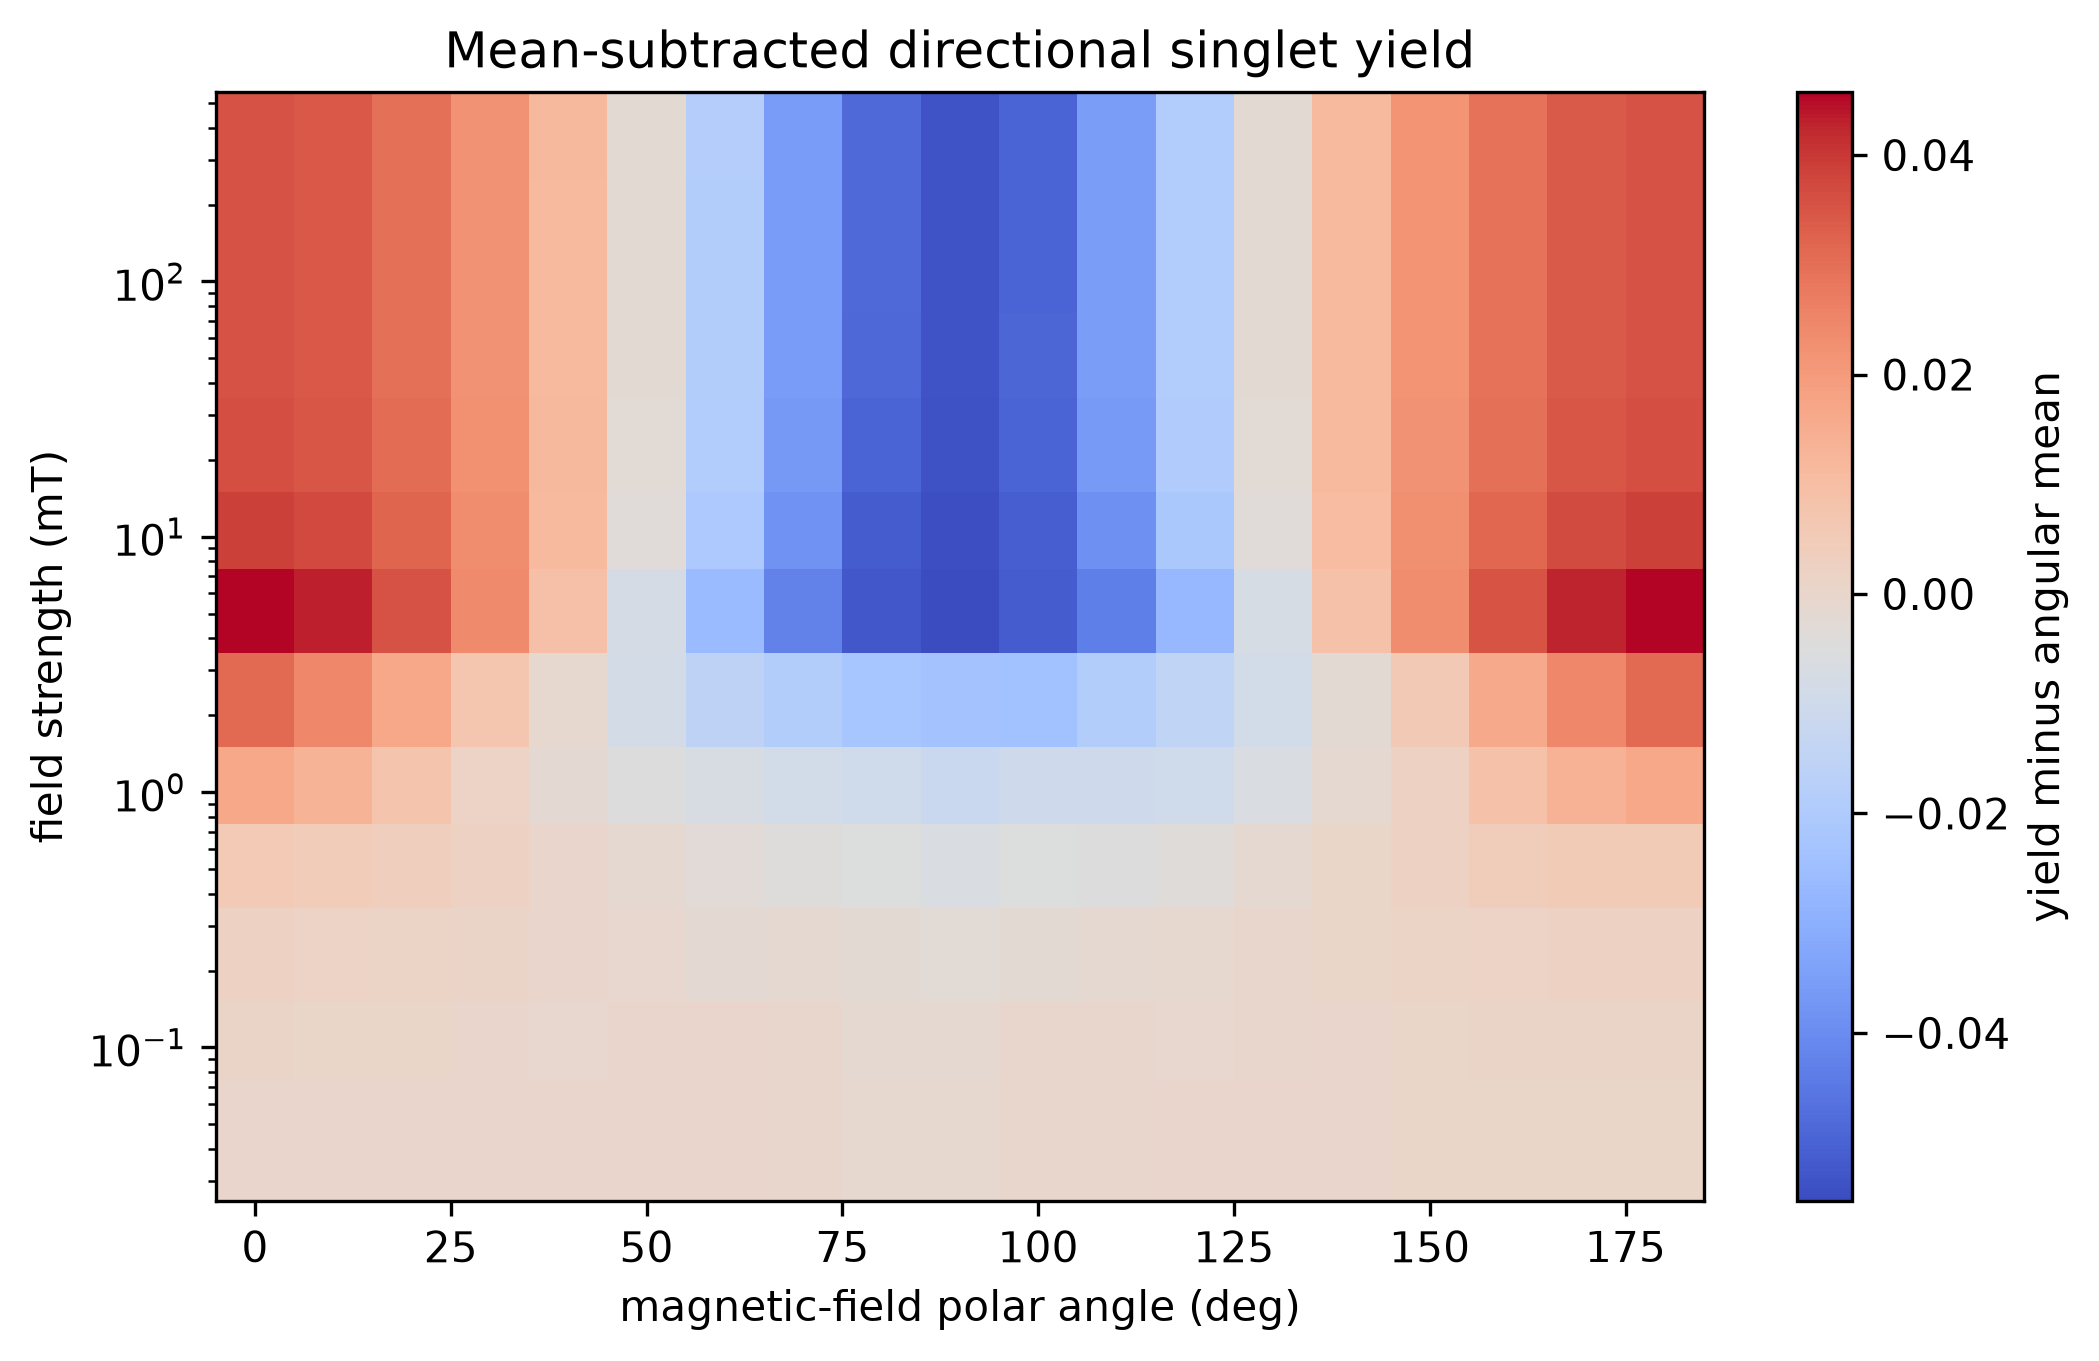
\includegraphics[width=\linewidth]{../figures/03-directional-heatmap.png}
    \caption{Directional yield heatmap.}
    \label{fig:directional-yield-heatmap}
\end{figure}
\subsection{Semiclassical Comparison}
We compare a full quantum mechanical treatment with two semiclassical approximations of the nuclear bath: a Gaussian static field and an atomwise static field. Both approximations produce static fields, but use different construction methods.

The Gaussian static approximation replaces all nuclei with a three-dimensional Gaussian random field. Its covariance exactly matches that of the quantum nuclei, but higher-order moments are discarded.

\noindent\textbf{Gaussian static distribution:}

\begin{equation}
    \mathbf{b}_r \sim \mathcal{N}\!\left(\mathbf{0}, \boldsymbol{\Sigma}_r\right),
    \qquad
    \boldsymbol{\Sigma}_r
    = \sum_k \frac{I_k\left(I_k+1\right)}{3}\,
      \mathbf{A}_k\mathbf{A}_k^{T}.
    \label{eq:gaussian-static-field}
\end{equation}

The atomwise static approximation constructs the field nucleus by nucleus using:

\begin{equation}
    \mathbf{b}_r = \sum_k \mathbf{A}_k\mathbf{i}_k,
    \qquad
    \mathbf{i}_k = \sqrt{I_k\left(I_k+1\right)}\,\hat{\mathbf{n}}_k.
    \label{eq:atomwise-static-field}
\end{equation}

This model can be thought of as lying between the Gaussian field and a full quantum description. It retains each nucleus's quantum spin number, its individual hyperfine coupling, and the finite number of terms and non-Gaussian structure of the summed field. Importantly, the mean and covariance of both static fields are the same; they differ only in their higher moments. With many weakly coupled nuclei, the atomwise distribution should approach the Gaussian distribution by the central limit theorem. With only 14 anisotropically coupled nuclei, however, the two distributions need not be identical. Differences between the Gaussian and atomwise results therefore test whether the covariance alone describes the nuclear-field distribution, while differences between either static result and the full quantum result test the importance of genuinely quantum and dynamical nuclear effects.

% TODO: Better resolve the zoomed-in plots around 90 degrees in the weak-field limit.

\begin{figure}[H]
    \centering
    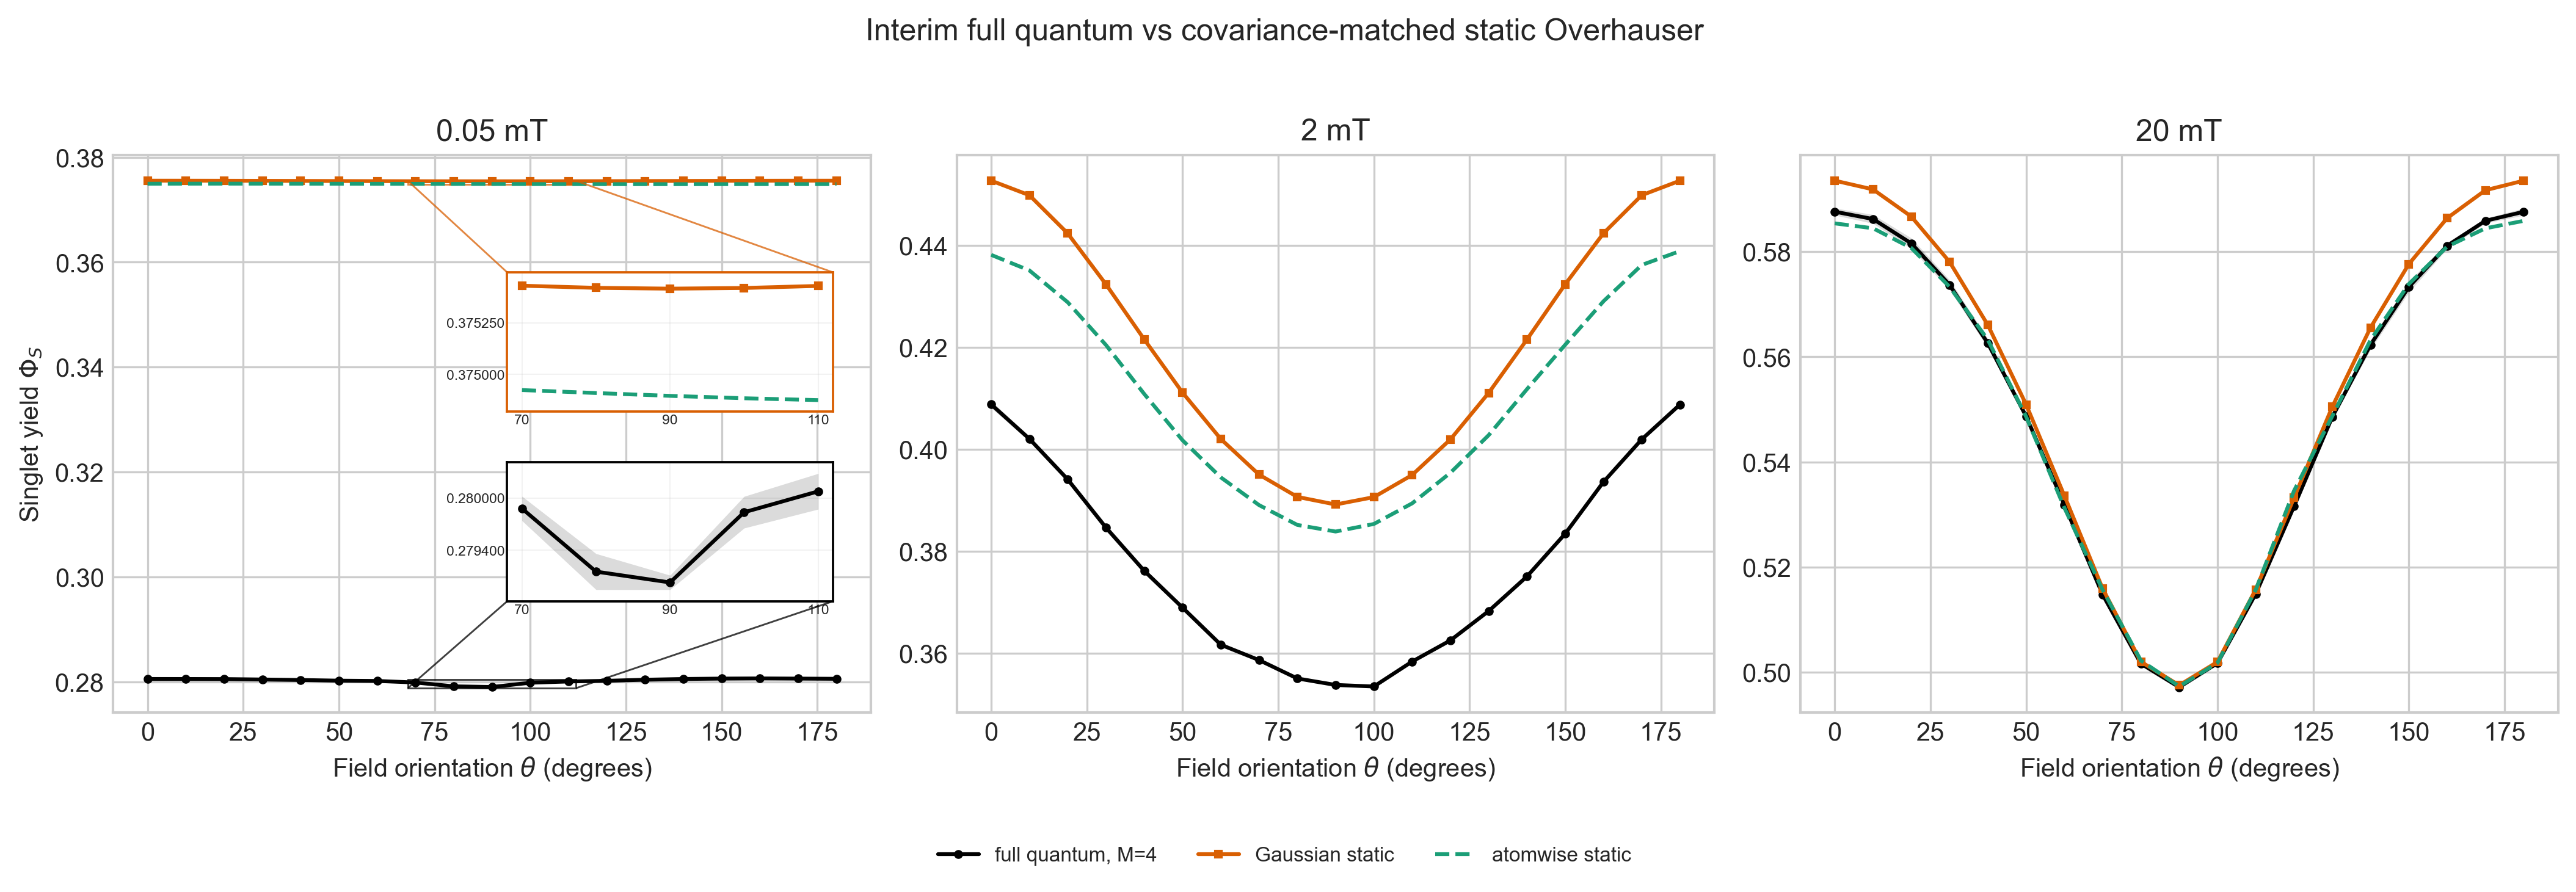
\includegraphics[width=\linewidth]{../figures/04-overhauser-comparison.png}
    \caption{Full quantum and covariance-matched static Overhauser comparison.}
    \label{fig:semiclassical-comparison}
\end{figure}
\subsection{Low to High Field Shift}
According to our models, we've now shown that as the external field stregnth grows, the nuclear environment's effect dimnishes, leading to a simpler model of the radical pair being drivewn by their axial coupling to the external magnetic field. This is in contrast with the geomagnetically relevant low field regime
where the theorized driver of the radical pair's magnetoreception is the transverse components in the anisotropic hyperfine interactions with the dominant Nitrogen nuclei in the FAD and Tryptophan molecules [refs]. Limited previous literature has simply noted that as the system's magnetosensitivity scales somewhat with these transverse coupling magnitudes [refs].
Since previous sections have shown a high field, electron axial driving regime, we hope to better understand what determines this shift from the low field, transverse to high field, axial driving. 
To this end, we adopt a toy model RPM to simplify the study of this shift. We use the toy RPM $[\mathrm{X}^{\bullet}\,\mathrm{Y}^{\bullet}]$ pair with $\tau = 10\,\mu\mathrm{s}$. $\mathrm{X}^{\bullet}$ carries an N5-like $^{14}\mathrm{N}$ tensor $(-0.0989, -0.0989, 1.7569)\,\mathrm{mT}$;
$\mathrm{Y}^{\bullet}$ is a purely axial Trp-N1-like $^{14}\mathrm{N}$ with tensor $(0, 0, 1.0812)\,\mathrm{mT}$. All transverse coupling therefore lives on
$\mathrm{X}^{\bullet}$.

We sweep $B_0$ from $0.05$ to $100\,\mathrm{mT}$ and rotate it through $\theta$. We track the singlet yield and define the diagnostic ablation fraction
\begin{equation}
    f = 1 - \frac{\Gamma_{\text{transverse zeroed}}}{\Gamma_{\text{full}}}.
\end{equation}
Thus, $f \approx 1$ indicates transverse driving, whereas $f \approx 0$ indicates that the transverse components are irrelevant. Exchange and dipolar electron and quadrupolar interactions are omitted.


\begin{figure}[H]
    \centering
    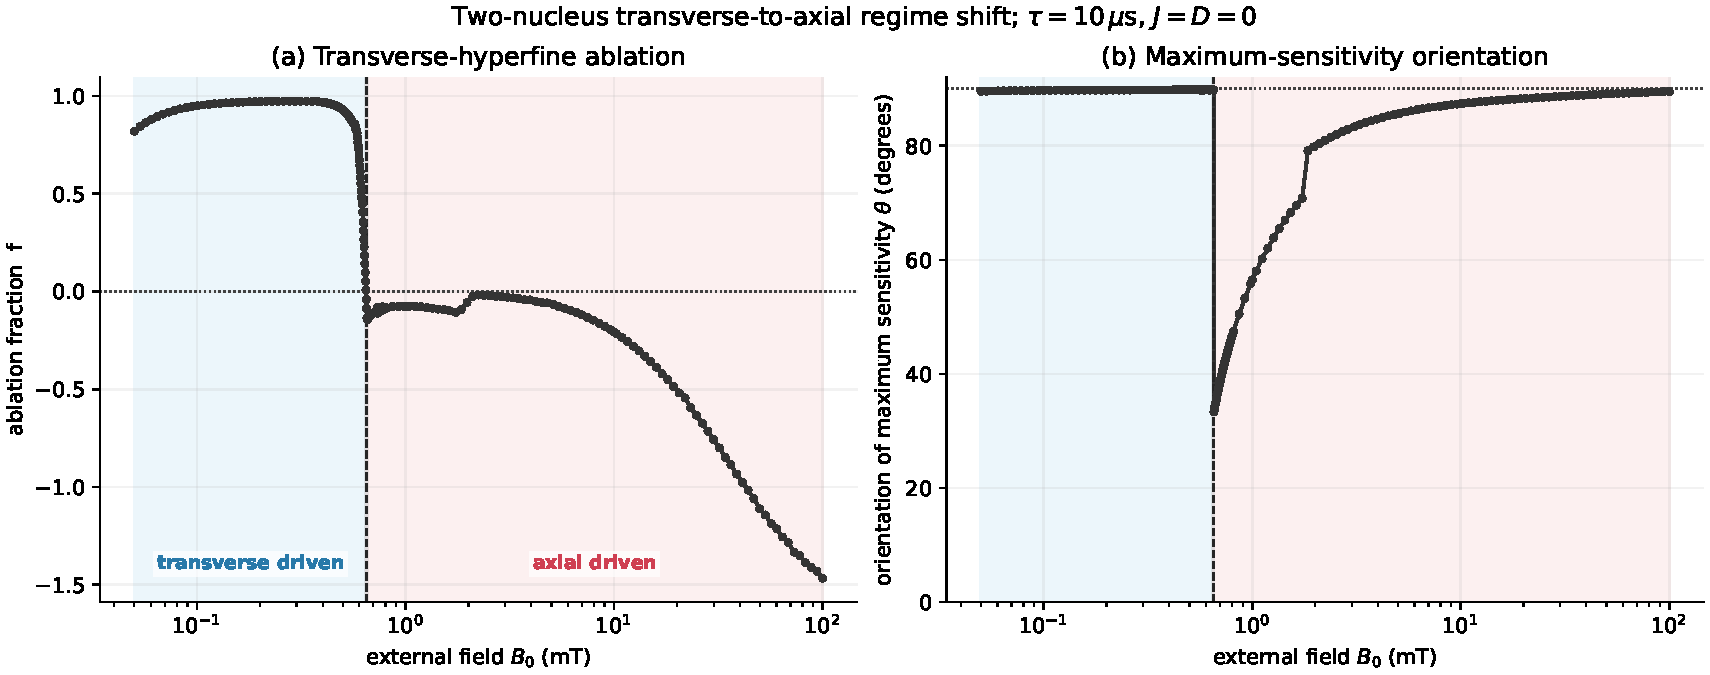
\includegraphics[width=\linewidth]{assets/regime_shift_refined_figure1.pdf}
    \caption{Regime change.}
    \label{fig:regime-change}
\end{figure}

Figure~\ref{fig:regime-change} shows that the two independent signatures flip together between $0.5$ and $0.7\,\mathrm{mT}$. Below the crossover, zeroing the transverse components destroys approximately $95\%$ of the angular sensitivity, and the sharp feature is locked at $\theta = 90^\circ$. Above it, removing them changes nothing---and at $100\,\mathrm{mT}$ the sensor performs better without them ($f = -1.23$), indicating that transverse coupling has become a blurring term. Simultaneously, the feature unpins from $90^\circ$, jumping to $38.6^\circ$ and then drifting back as $B_0$ rises.

The crossover scale seems to coincide with the dominant hyperfine, axial coupling ($A_{zz}/3$), not the transverse coupling, nor the axial, external field coupling to the electron spins.
\subsection{Low Field Optimum}
The results from Figure~\ref{fig:regime-change} suggest that there must be a low-field optimum for the angular sensitivity of the sensor. To better understand this optimum , we track the amplitude and sensitivity of the peak angular response as a function of the transverse coupling and coherence time.

\paragraph{Experimental setup.}
\begin{itemize}
    \item We use the same two-nucleus system. The parameter $\lambda$ scales only the transverse components, while $A_{zz}$ is held fixed. The control variable is the physical transverse coupling
    \begin{equation}
        b = \gamma_e \sqrt{A_{xx}^{2} + A_{yy}^{2}}.
    \end{equation}
    \item For $\lambda = 1$, $b = 140\,\mu\mathrm{T}$. The physical N5 coupling lies at $\lambda \approx 0.95$, corresponding to $b = 133\,\mu\mathrm{T}$---already approximately $2.7$ times Earth's field.
    \item We fix $B_0 = 50\,\mu\mathrm{T}$ and evaluate $17$ values of $\lambda$ for each $\tau \in \{1, 10, 100\}\,\mu\mathrm{s}$. The singlet yield $\Phi_S$ is calculated exactly, without approximation.
    \item The validation gates are satisfied: $\Phi_S(H = 0) = 1.000000$; the spike vanishes identically at zero transverse coupling, confirming a true level crossing; and the spike deepens as $\tau$ increases.
\end{itemize}

\paragraph{Result.}
There is an interior optimum: both amplitude and sensitivity initially rise and then fall. The optimum occurs at several times Earth's field and shifts with $\tau$, revealing a transverse-coupling--coherence-time trade-off.

\begin{figure}[H]
    \centering
    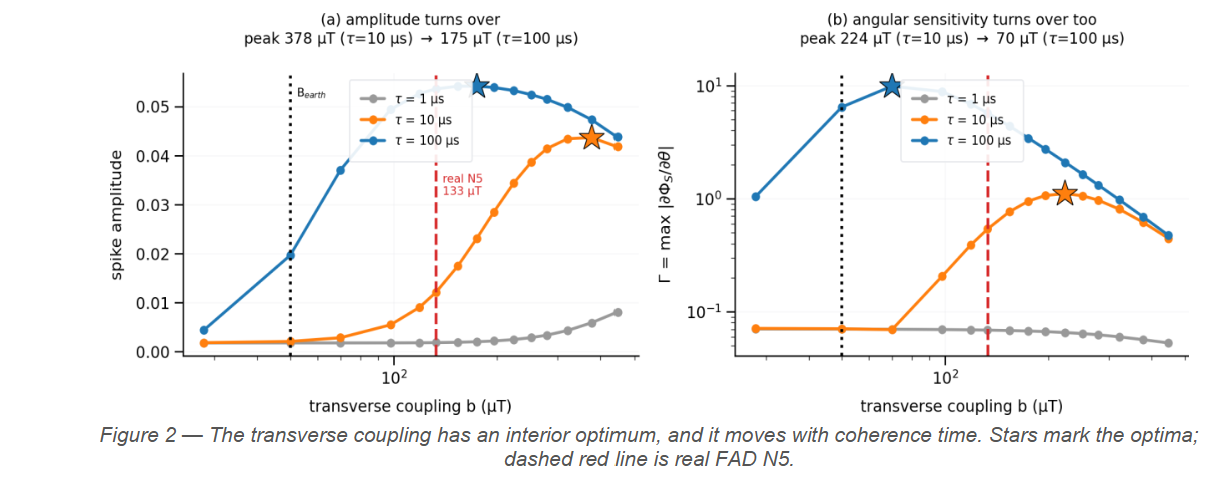
\includegraphics[width=\linewidth]{../figures/06-transverse-optimum.png}
    \caption{Low-field optimum.}
    \label{fig:low-field-optimum}
\end{figure}

\subsection{Optimum Scaling Law}
The optimum moving systematically with $\tau$ suggested a law rather than a coincidence, so we mapped the optimum transverse coupling for angular sensitivity, $b_{\mathrm{opt}}(\tau)$, across three axial couplings to further explore the relationship between axial and transverse couplings.

\paragraph{Experimental setup.}
\begin{itemize}
    \item For each axial-hyperfine-and-coherence-time cell, $(A_{zz}, \tau)$, we sweep $b$, compute $\Gamma = \max \lvert \partial \Phi_S / \partial \theta \rvert$ at each $b$, and take the argmax. This gives $3 \times 5 = 15$ cells.
    \item $A_{zz} \in \{0.6046, 1.2, 1.7569\}\,\mathrm{mT}$, corresponding to real FAD N10, a synthetic midpoint, and real FAD N5, respectively; $\tau \in \{5, 10, 20, 50, 100\}\,\mu\mathrm{s}$.
    \item This tracks the sensitivity optimum, not the amplitude optimum; only the sensitivity branch obeys a clean law.
\end{itemize}

\paragraph{Result---the scaling law.}
\begin{equation}
    b_{\mathrm{opt}} = C\,\frac{A_{zz}}{\sqrt{\tau}},
    \qquad
    C \approx 391\,\frac{\mu\mathrm{T}\sqrt{\mu\mathrm{s}}}{\mathrm{mT}}.
\end{equation}
Normalising by $A_{zz}$ collapses a threefold range of axial coupling onto a single curve, agreeing to four decimal places. The raw $b_{\mathrm{opt}}$ values at $\tau = 10\,\mu\mathrm{s}$ differ by a factor of three: $75.2$, $149.1$, and $218.3\,\mu\mathrm{T}$. The fitted exponents are $-0.4952$, $-0.4954$, and $-0.4955$, so the $-1/2$ exponent holds to approximately $1\%$, with an approximately $2\%$ residual drift in $C$ across the $\tau$ range. $A_{zz}$ sets the scale and nothing else does.

Inverting the law for $b = 132.5\,\mu\mathrm{T}$ gives $\tau \approx 29\,\mu\mathrm{s}$. Running the $\Gamma$ sweep at that lifetime, real FAD N5 lands at $100.0\%$ of peak.


\begin{figure}[H]
    \centering
    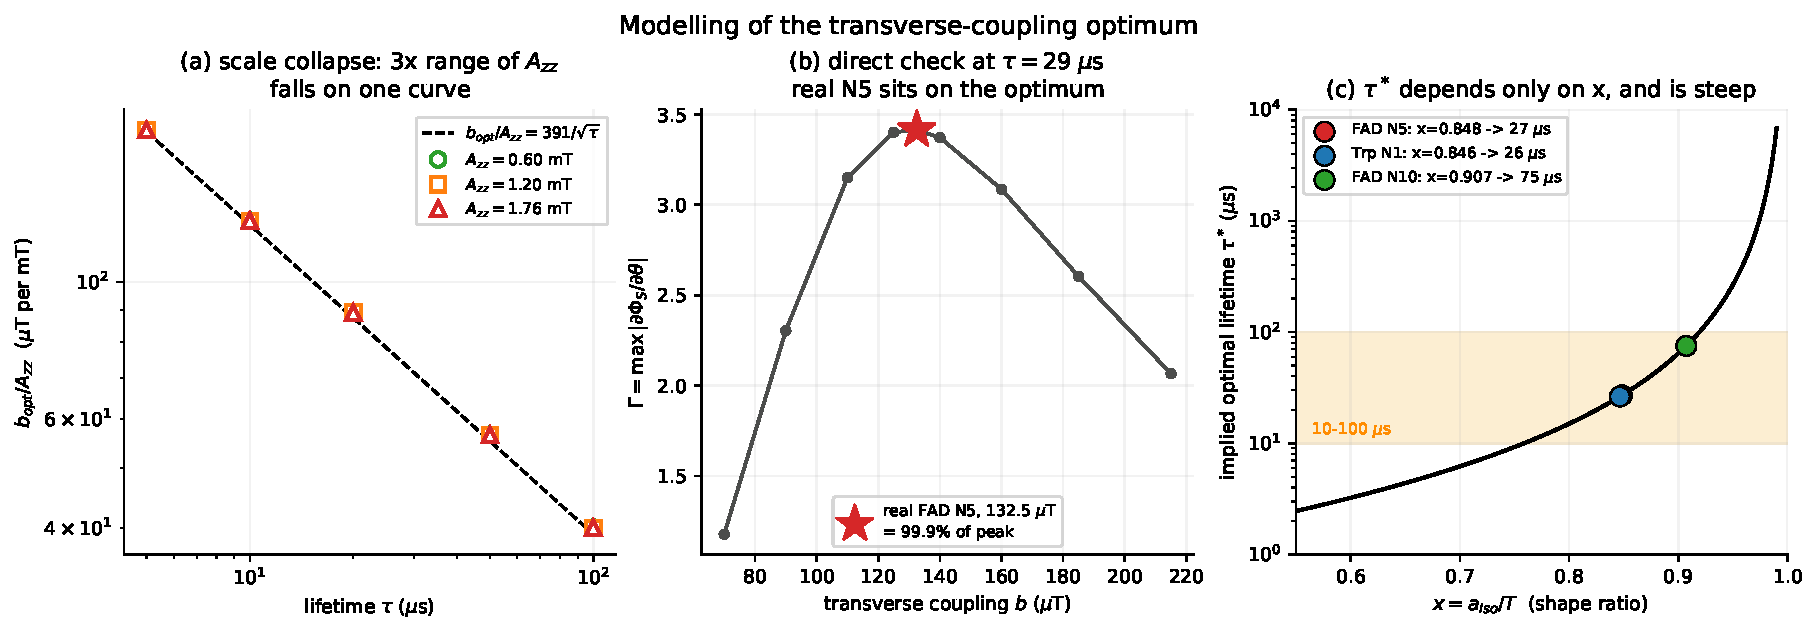
\includegraphics[width=\linewidth]{assets/section3_modelling_the_optimum.pdf}
    \caption{Scaling law.}
    \label{fig:scaling-law}
\end{figure}

We have now developed a scaling law that describes the motion of the optimal transverse coupling with coherence time and shown that this scaling is determined purely by the axial hyperfine coupling, $A_{zz}$. We now link the chemical shape of aromatic nitrogens to this axial--transverse coupling relationship to show that this chemical shape factor alone can describe the optimal angular sensitivity of the radical-pair singlet yield.

\paragraph{Why this connects to aromatic nitrogen:}
\[
\hat{H}_{\mathrm{hf}}
=
\hat{\mathbf{S}} \cdot \mathbf{A} \cdot \hat{\mathbf{I}}
\]

\[
\mathbf{A}
=
a_{\mathrm{iso}}\,\mathbf{1}
+
T
\begin{pmatrix}
-1 & 0 & 0 \\
0 & -1 & 0 \\
0 & 0 & 2
\end{pmatrix}
\]
Writing the tensor in axial form,
\begin{equation}
    A_{zz} = a_{\mathrm{iso}} + 2T,
    \qquad
    b = \sqrt{2}\,\lvert a_{\mathrm{iso}} - T \rvert.
\end{equation}
Setting the real $b$ equal to the optimal $b$ and solving for the lifetime, $T$ cancels, leaving
\begin{equation}
    \tau^{*}(x) = \left[\frac{k(x + 2)}{\sqrt{2}\,\lvert x - 1 \rvert}\right]^{2},
\end{equation}
with $x = a_{\mathrm{iso}}/T$ and $k = C/1000$, where $x$ is the tensor shape. 

\begin{table}[H]
    \centering
    \caption{Tensor shape and implied optimal lifetime for the dominant aromatic nitrogens.}
    \label{tab:aromatic-nitrogen-tensor-shape}
    \small
    \renewcommand{\arraystretch}{1.2}
    \begin{tabular}{|l|c|c|c|c|}
        \hline
        \rowcolor{black!8}
        \textbf{Nucleus} & $a_{\mathrm{iso}}$ (mT) & $T$ (mT) & $x = a_{\mathrm{iso}}/T$ & Implied $\tau^{*}$ ($\mu\mathrm{s}$) \\
        \hline
        FAD N5 & 0.5233 & 0.6168 & 0.848 & 27 \\
        \hline
        Trp N1 & 0.3215 & 0.3798 & 0.847 & 26 \\
        \hline
        FAD N10 & 0.1887 & 0.2080 & 0.907 & 76 \\
        \hline
    \end{tabular}
\end{table}

All three dominant, anisotropic nitrogens in the RPM (FAD: N5, N10 and Trp:N1) are $\pi$-conjugated $\mathrm{sp}^{2}$
 aromatic nitrogens and all three share $x \approx 0.85\text{--}0.91$---the unpaired spin density sits in a $p_z$ orbital,
  which fixes the dipolar term relative to the contact term. Table \ref{tab:aromatic-nitrogen-tensor-shape} shows that we expect an optimal coherence time in the tens-of-$\mu\mathrm{s}$ range 
  for each of these nitrogrens. This promotes previous work showing that the RPM responsible for avian magnetoreception would need coherence times 5-100 $\mu\mathrm{s}$ [ref] and the optimality of these coherence times is purely a consequence of
   aromatic nitrogen chemistry.


\subsection{Nuclear Spin Control}
\begin{figure}[H]
    \centering
    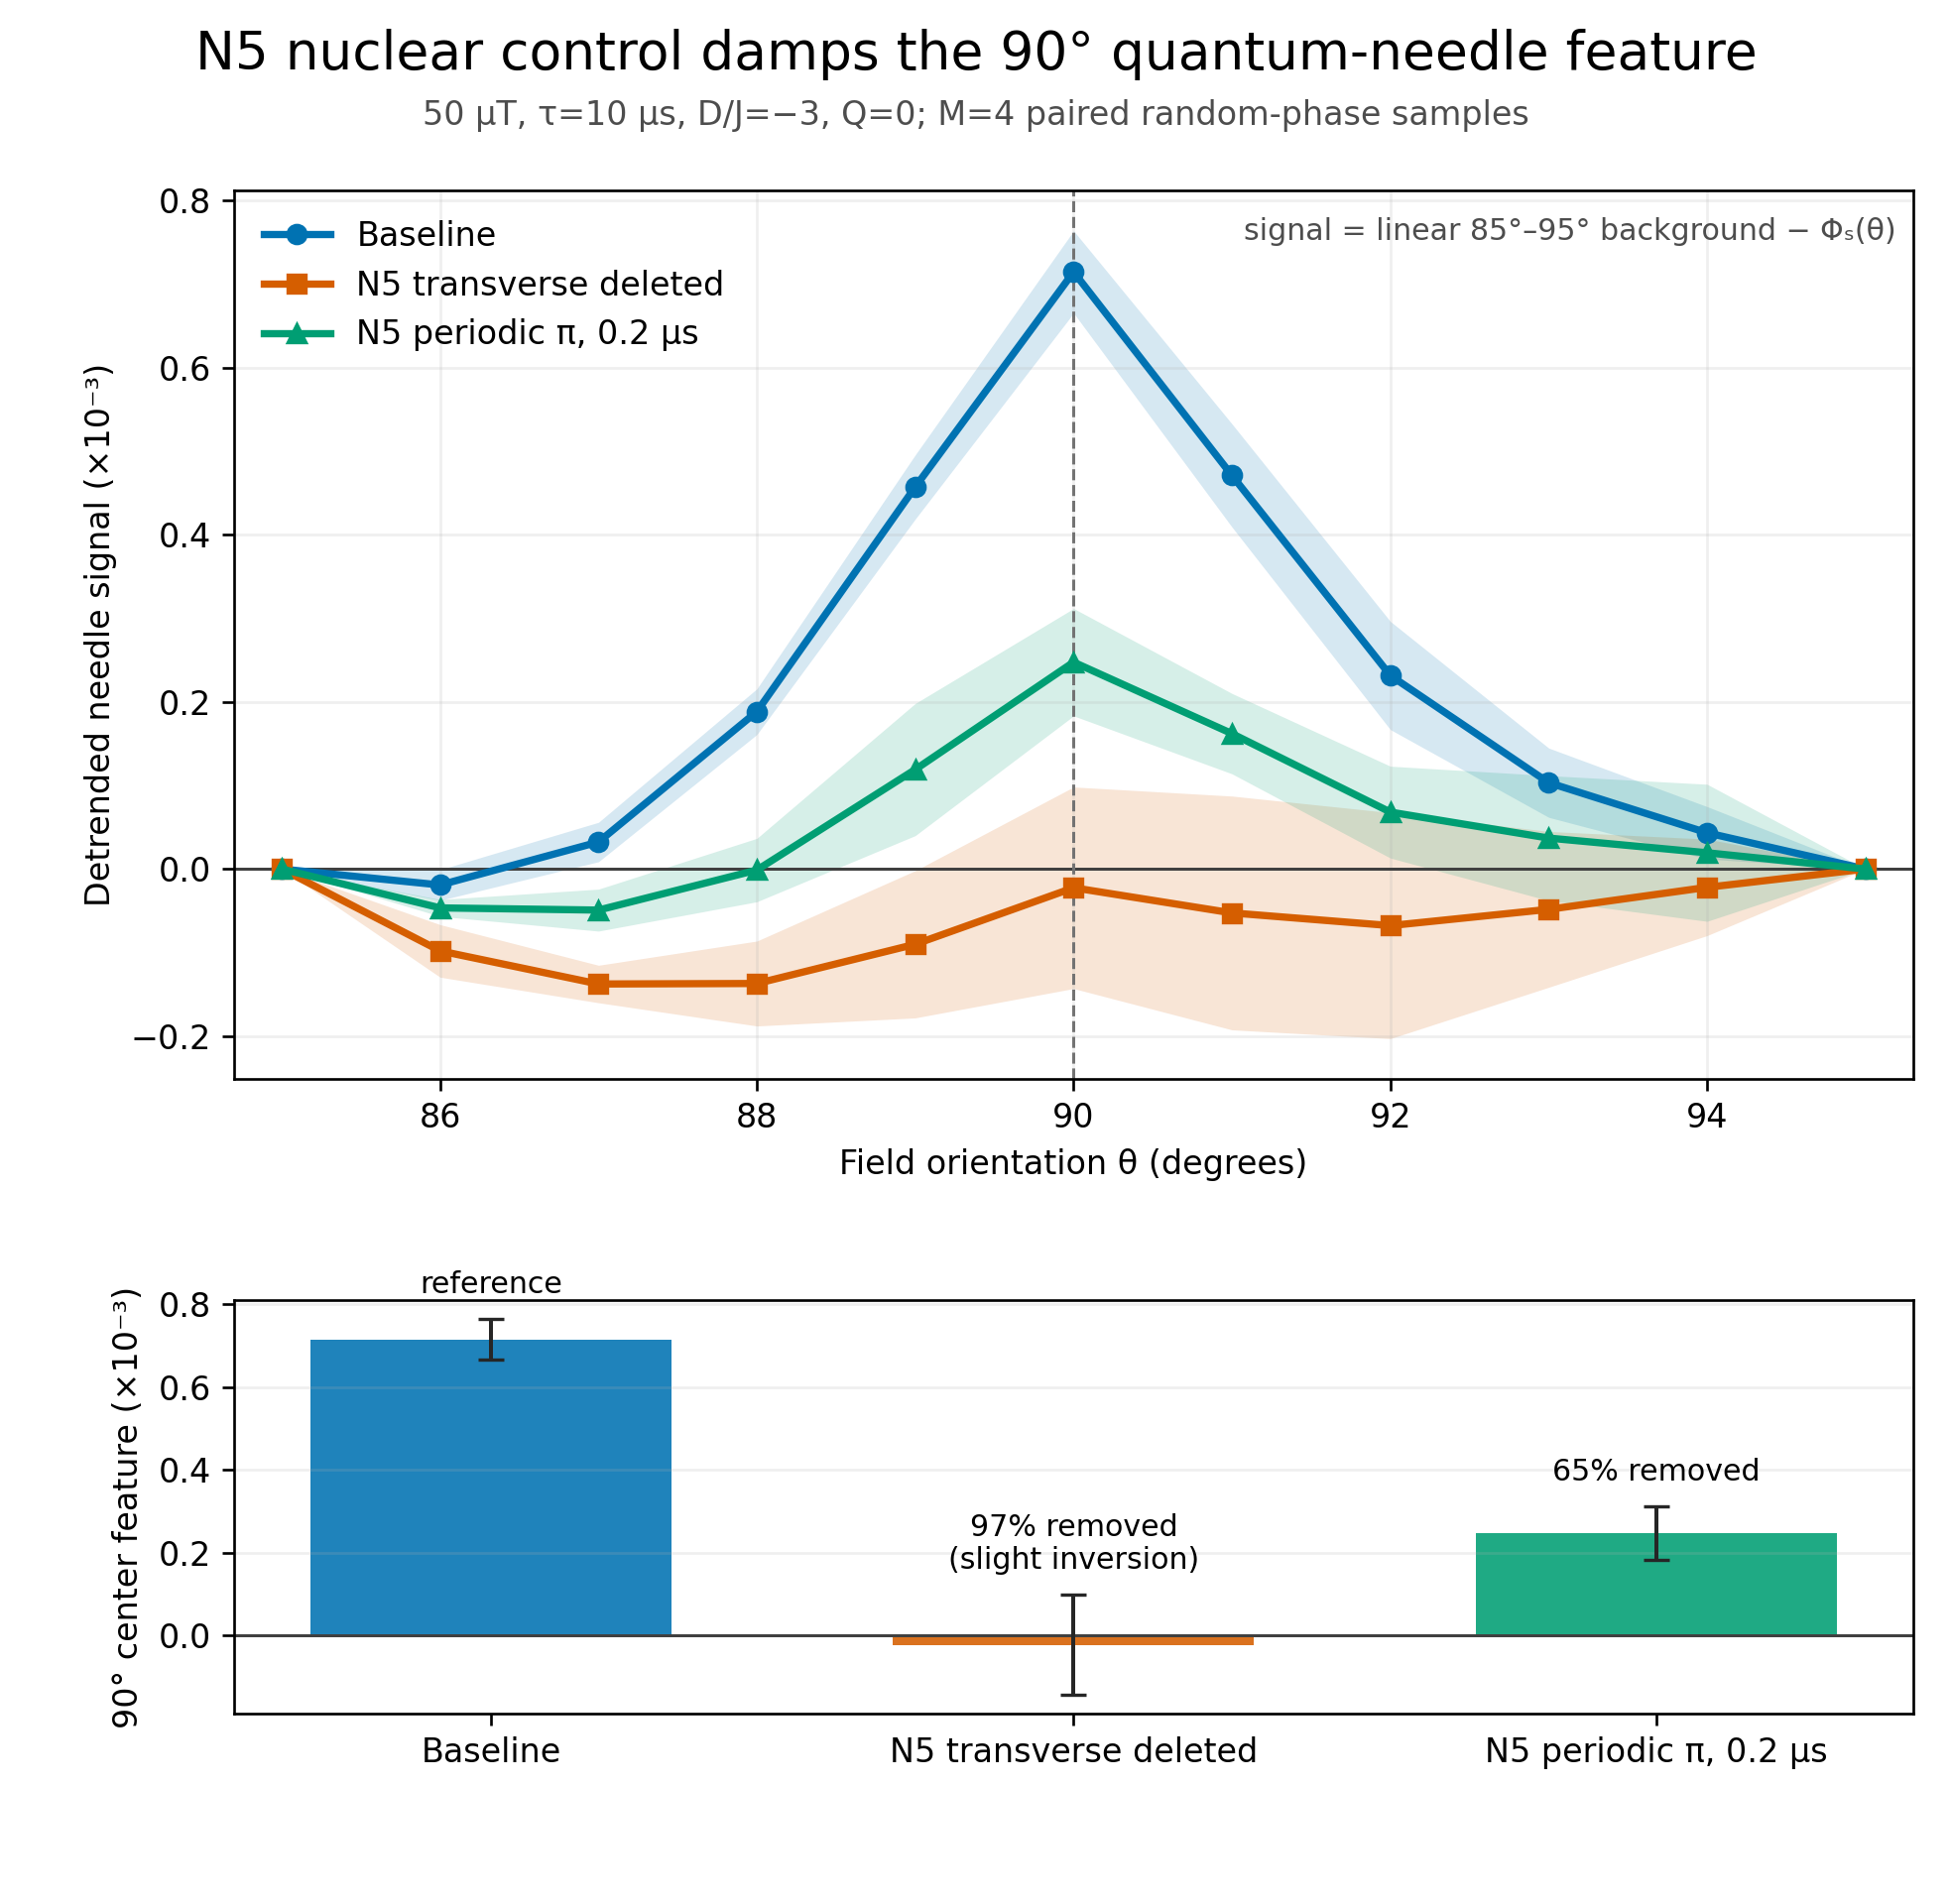
\includegraphics[width=\linewidth]{../figures/08-n5-spin-control.png}
    \caption{Detrended N5 nuclear-spin control needle.}
    \label{fig:n5-control-needle-detrended}
\end{figure}
\subsection{Entanglement and Magic}
We track logarithmic negativity across two subsystem cuts: Cut~1 separates the radicals, and Cut~2 separates the electron pair from the nuclear environment. We explicitly track systems with up to 14 nuclei (seven per radical), then use a power-law extrapolation to extend the scaling to each radical's nuclear environment. The dotted orange line in the left plot and dotted grey line in the right plot mark the theoretical maxima for each system size. These coherent, closed-system dynamics represent highly idealized conditions for entanglement.

\begin{figure}[H]
    \centering
    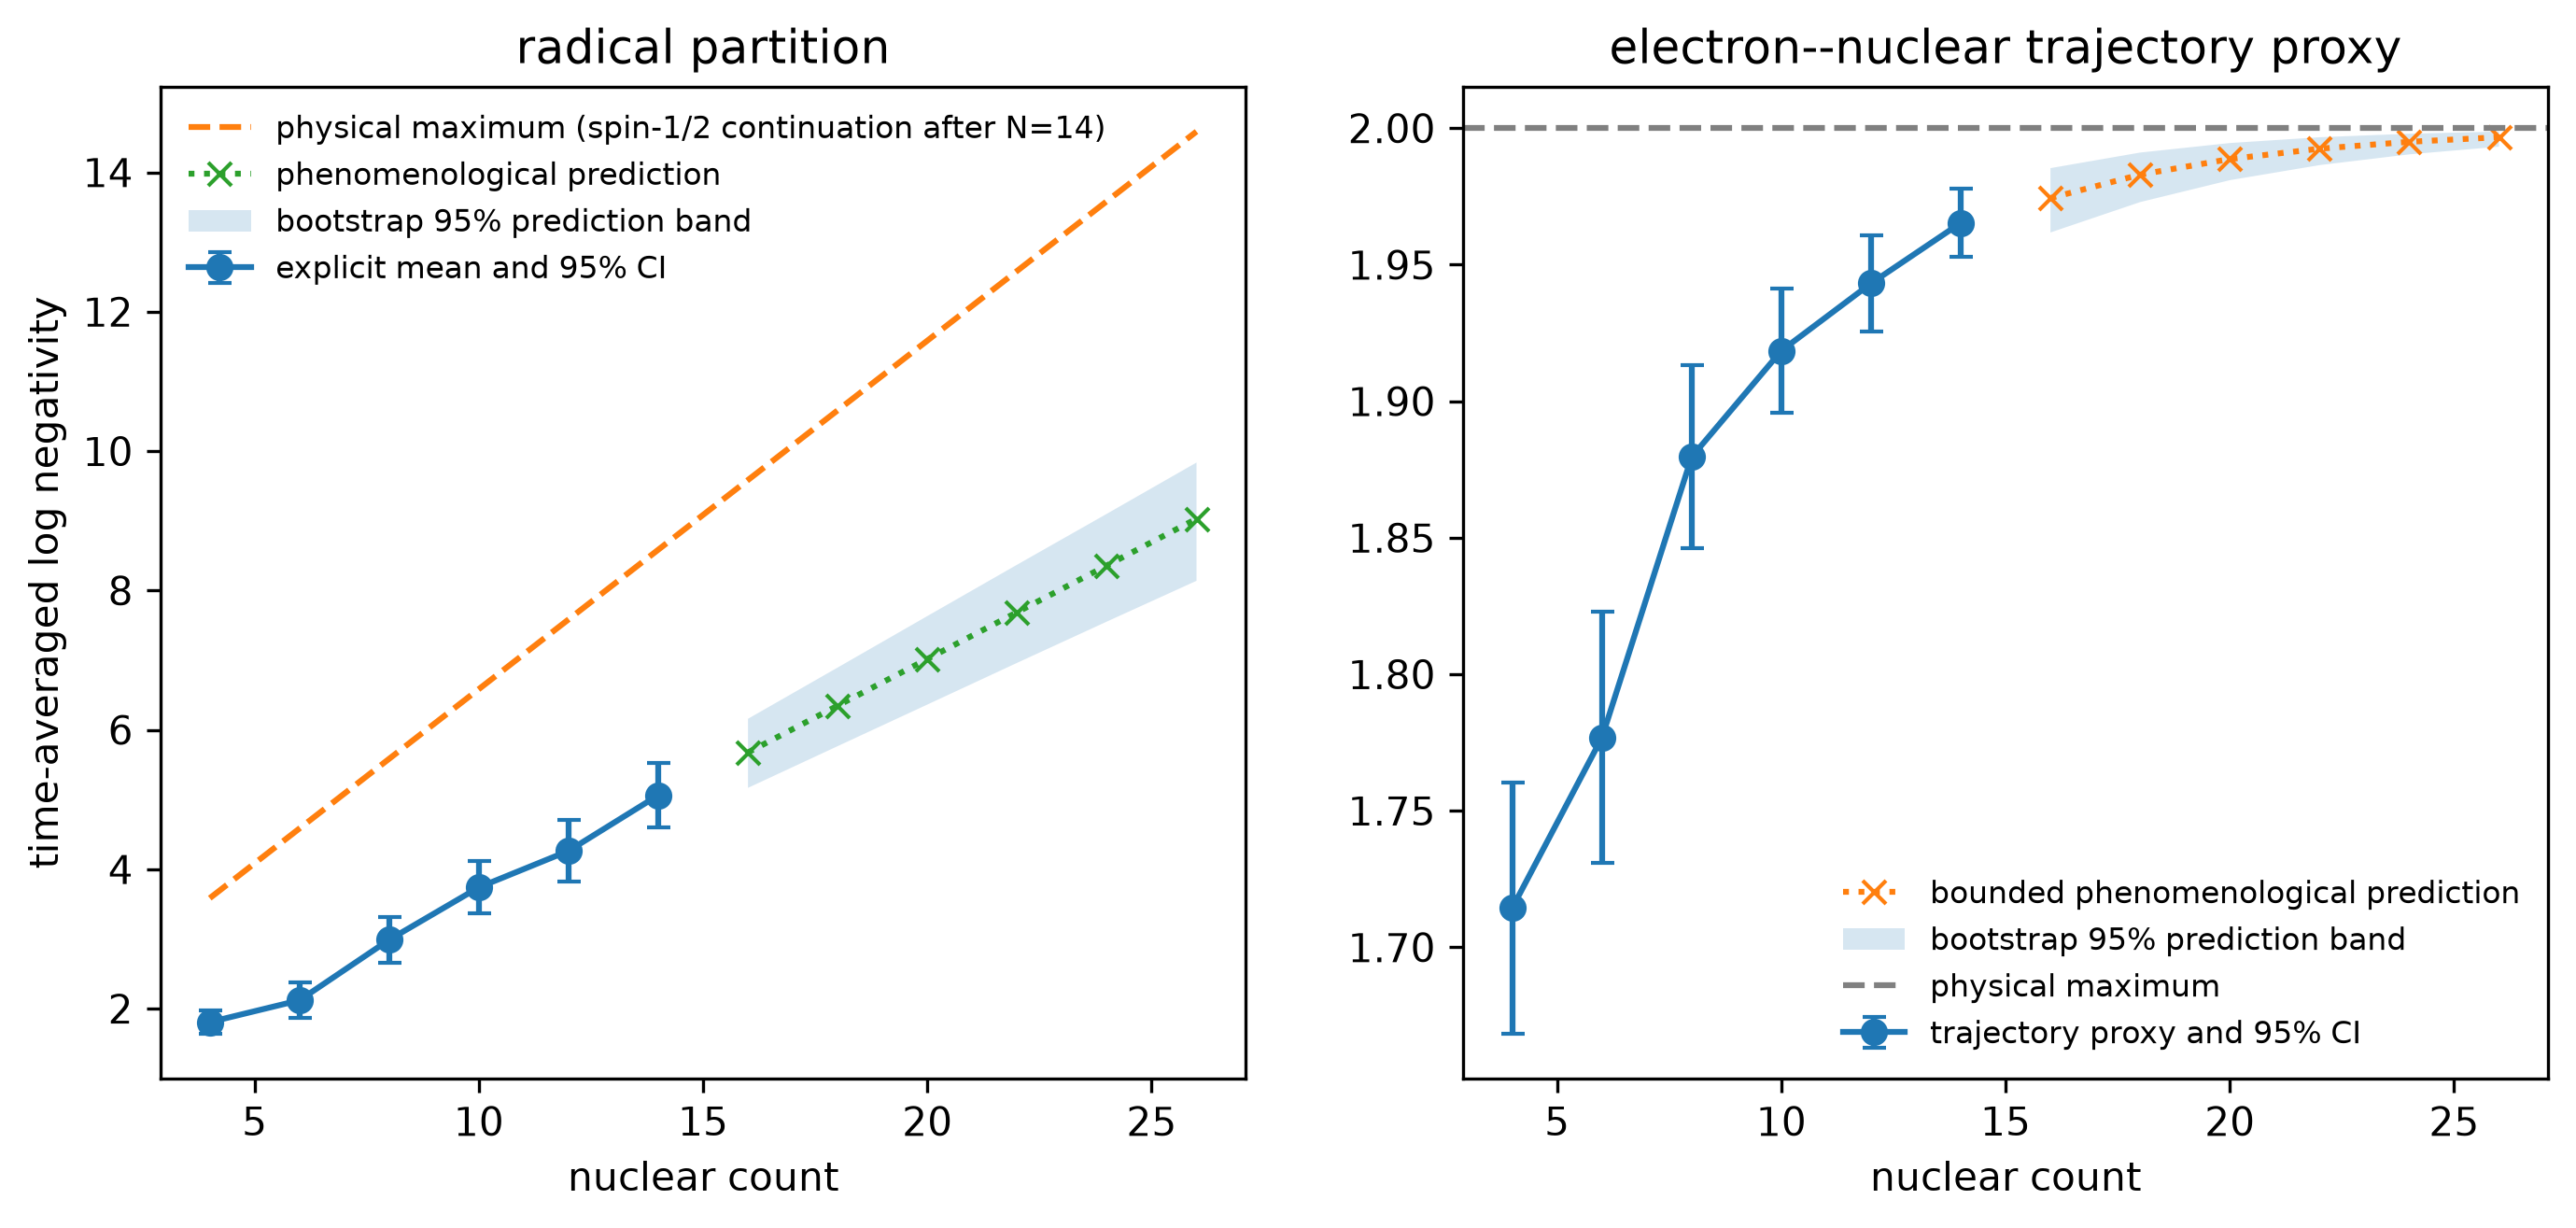
\includegraphics[width=\linewidth]{../figures/09-entanglement-scaling.png}
    \caption{Entanglement scaling.}
    \label{fig:entanglement-scaling}
\end{figure}
\begin{figure}[H]
    \centering
    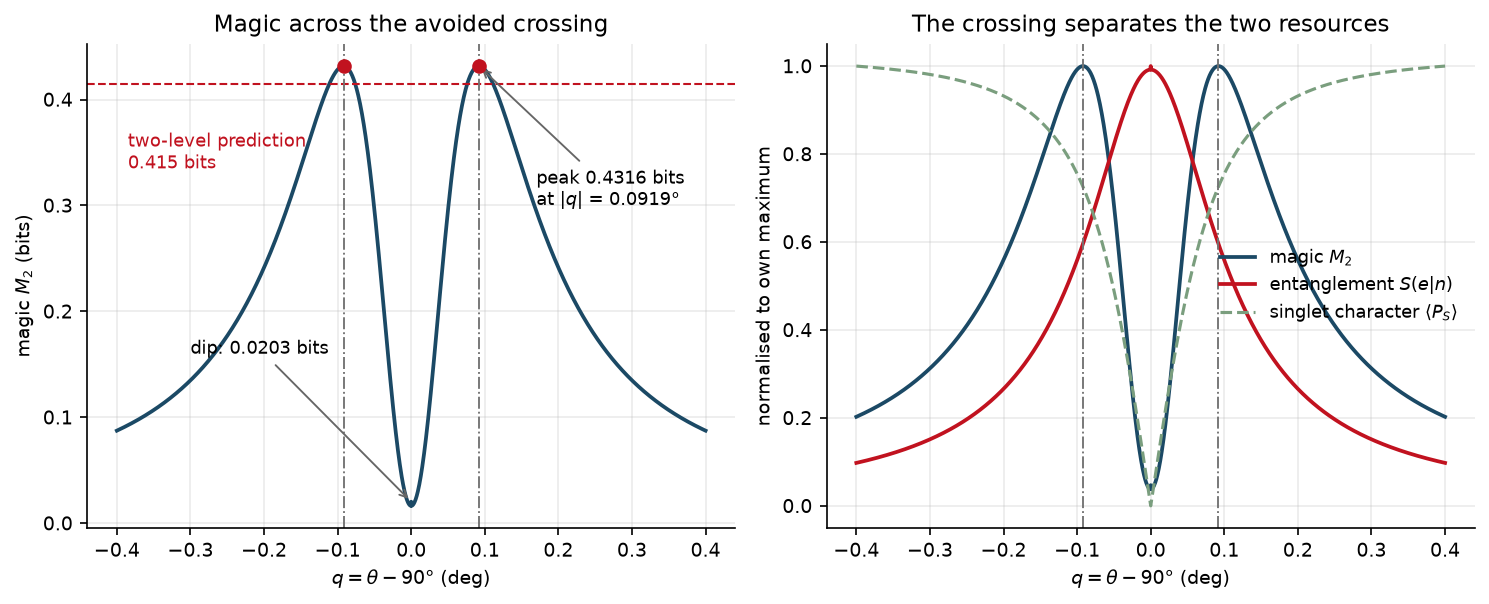
\includegraphics[width=\linewidth]{../figures/10-magic-entanglement.png}
    \caption{Radical-pair magic and entanglement.}
    \label{fig:rpm-magic-entanglement}
\end{figure}
\end{document}
